% ---- pgfplots style ----
\definecolor{cfifo}{HTML}{2A78D6}\definecolor{clru}{HTML}{EB6834}
\pgfplotsset{compat=1.18,
  every axis/.append style={font=\footnotesize, axis lines=left, grid=major, major grid style={black!10},
    title style={font=\small\sffamily\color{navy}}, legend style={draw=none, fill=white, fill opacity=0.85, text opacity=1, font=\footnotesize},
    tick align=outside, axis line style={black!45}},
  fifo/.style={cfifo, line width=1.4pt, mark=*, mark size=2pt, mark options={fill=white, line width=1pt}},
  lru/.style={clru, line width=1.4pt, mark=square*, mark size=2pt, mark options={fill=white, line width=1pt}}}
\newcommand{\plotLocality}[1][0.48\linewidth]{%
\begin{tikzpicture}\begin{axis}[width=#1, height=0.62*#1, xmode=log, log basis x=2, xtick={8,16,32,64,128,256}, xticklabels={8,16,32,64,128,256},
 title={Locality өгөгдөл (1000 хаяг)}, xlabel={Frame-ийн тоо}, ylabel={Page fault rate, \%}, ymin=10,ymax=52]
\addplot[fifo] coordinates {(8,47.8) (16,27.7) (32,21.4) (64,19.3) (128,16.6) (256,16.1)}; \addlegendentry{FIFO}
\addplot[lru] coordinates {(8,44.5) (16,22.6) (32,21.0) (64,19.2) (128,16.6) (256,16.1)}; \addlegendentry{LRU}
\end{axis}\end{tikzpicture}}
\newcommand{\plotBook}[1][0.48\linewidth]{%
\begin{tikzpicture}\begin{axis}[width=#1, height=0.62*#1, xmode=log, log basis x=2, xtick={8,16,32,64,128,256}, xticklabels={8,16,32,64,128,256},
 title={Номын addresses.txt (1000 хаяг)}, xlabel={Frame-ийн тоо}, ylabel={Page fault rate, \%}, ymin=20,ymax=100]
\addplot[fifo] coordinates {(8,97.5) (16,94.6) (32,88.2) (64,76.2) (128,53.8) (256,24.4)}; \addlegendentry{FIFO}
\addplot[lru] coordinates {(8,97.5) (16,94.5) (32,87.9) (64,75.4) (128,53.9) (256,24.4)}; \addlegendentry{LRU}
\node[font=\scriptsize, navy, anchor=north east, align=right] at (axis cs:256,40) {256 frame: 244 fault\\= ялгаатай page-ийн тоо};
\end{axis}\end{tikzpicture}}
\newcommand{\plotTLB}[1][0.48\linewidth]{%
\begin{tikzpicture}\begin{axis}[width=#1, height=0.62*#1, xmode=log, log basis x=2, xtick={1,2,4,8,16,32,64}, xticklabels={1,2,4,8,16,32,64},
 title={TLB hit rate (locality, 256 frame)}, xlabel={TLB-ийн хэмжээ}, ylabel={TLB hit rate, \%}, ymin=0,ymax=90,legend pos=south east]
\addplot[fifo] coordinates {(1,9.8) (2,18.5) (4,31.9) (8,52.2) (16,72.3) (32,78.6) (64,80.7)}; \addlegendentry{FIFO}
\addplot[lru] coordinates {(1,9.8) (2,18.2) (4,33.2) (8,55.5) (16,77.4) (32,79.0) (64,80.8)}; \addlegendentry{LRU}
\end{axis}\end{tikzpicture}}
\newcommand{\plotBelady}[1][0.48\linewidth]{%
\begin{tikzpicture}\begin{axis}[width=#1, height=0.62*#1, xtick={1,2,3,4,5,6}, xticklabels={1,2,3,4,5,6},
 title={Belady: 1 2 3 4 1 2 5 1 2 3 4 5}, xlabel={Frame-ийн тоо}, ylabel={Page fault}, ymin=0,ymax=13,legend pos=south west]
\addplot[fifo] coordinates {(1,12) (2,12) (3,9) (4,10) (5,5) (6,5)}; \addlegendentry{FIFO}
\addplot[lru] coordinates {(1,12) (2,12) (3,10) (4,8) (5,5) (6,5)}; \addlegendentry{LRU}
\draw[navy, line width=0.6pt] (axis cs:4,10) circle (5pt);
\node[font=\scriptsize, navy, anchor=south west, align=left] at (axis cs:4.15,10.4) {FIFO: 3→4 frame үед\\fault 9→10 өссөн};
\end{axis}\end{tikzpicture}}


% ---- Гол үр дүнгийн хайрцаг ----
\newcommand{\stat}[2]{\begin{minipage}[t]{0.235\linewidth}\centering{\sffamily\LARGE\color{navy}\textbf{#1}}\\[2pt]{\footnotesize #2}\end{minipage}}
\newcommand{\keyresults}{%
\begin{tcolorbox}[colback=hblue!6, colframe=hblue!60, boxrule=0.6pt, arc=2pt, left=4pt, right=4pt, top=6pt, bottom=6pt,
  title={\sffamily Гол үр дүн}, coltitle=white, colbacktitle=navy, fonttitle=\small]
\stat{1000/1000}{Номын correct.txt-тэй\\таарсан мөр (256 frame)}\hfill
\stat{15 / 12}{Номын жишээ: FIFO / LRU\\fault (номтой таарсан)}\hfill
\stat{9 → 10}{Belady-ийн аномали\\(FIFO, 3 → 4 frame)}\hfill
\stat{22.6\%}{LRU fault rate (16 frame)\\FIFO-д 27.7\%}
\end{tcolorbox}}

% ---- Хаяг задлах диаграм (16916) ----
\newcommand{\addrsplit}{%
\begin{tikzpicture}[font=\footnotesize, bit/.style={draw=black!50, minimum width=6.2mm, minimum height=7mm, inner sep=0pt, font=\ttfamily}]
\node[anchor=east, font=\small] at (-0.15,0.35) {16916 =};
\foreach \b [count=\i from 0] in {0,1,0,0,0,0,1,0}
  \node[bit, fill=hblue!25, anchor=south west] at (\i*0.62,0) {\b};
\foreach \b [count=\i from 8] in {0,0,0,1,0,1,0,0}
  \node[bit, fill=clru!22, anchor=south west] at (\i*0.62,0) {\b};
\draw[decorate, decoration={brace, amplitude=5pt, mirror}, thick, navy] (0,-0.08) -- (4.96,-0.08)
  node[midway, below=6pt, align=center] {\textbf{page} = 0100 0010$_2$ = \textbf{66}\\(дээд 8 бит: \texttt{a >> 8})};
\draw[decorate, decoration={brace, amplitude=5pt, mirror}, thick, clru!80!black] (4.96,-0.08) -- (9.92,-0.08)
  node[midway, below=6pt, align=center] {\textbf{offset} = 0001 0100$_2$ = \textbf{20}\\(доод 8 бит: \texttt{a \& 0xFF})};
\node[anchor=west, align=left, font=\small] at (10.3,0.35) {page 66 → frame 0\\физик = 0×256 + 20 = \textbf{20}};
\node[font=\scriptsize, black!60] at (0.31,0.95) {15}; \node[font=\scriptsize, black!60] at (9.61,0.95) {0};
\end{tikzpicture}}

% ---- Хаяг хөрвүүлэх урсгал ----
\newcommand{\translationflow}{%
\begin{tikzpicture}[font=\footnotesize, >={Stealth[length=2mm]},
  b/.style={draw=navy, rounded corners=2pt, fill=hblue!8, align=center, inner sep=4pt, minimum height=9mm},
  d/.style={draw=navy, diamond, aspect=2.2, fill=white, align=center, inner sep=1pt},
  lab/.style={font=\scriptsize\itshape, black!70}]
\node[b] (cpu) at (0,0) {Логик хаяг\\\texttt{page | offset}};
\node[d] (tlb) at (3.6,0) {TLB-д\\байна уу?};
\node[d] (pt) at (3.6,-2.3) {page\_table\\$\neq -1$?};
\node[b, fill=rd!12, draw=rd] (pf) at (3.6,-4.4) {\textbf{Page fault}\\хоосон frame эсвэл\\FIFO/LRU victim};
\node[b] (bs) at (-0.9,-4.4) {Backing store\\(256 байт уншина)};
\node[b] (upd) at (7.6,-3.3) {page\_table ба TLB-г\\шинэчилнэ (victim-ийг\\хүчингүй болгоно)};
\node[b, fill=grn!12, draw=grn] (fr) at (7.6,0) {\textbf{frame}};
\node[b] (pa) at (11.2,0) {Физик хаяг\\frame×256 + offset};
\draw[->] (cpu)--(tlb);
\draw[->, grn!70!black, thick] (tlb)--node[above, lab]{hit}(fr);
\draw[->] (tlb)--node[right, lab]{miss}(pt);
\draw[->] (pt.east) -| node[pos=0.25, above, lab]{тийм} ([xshift=-6mm]fr.south);
\draw[->, rd] (pt)--node[right, lab]{үгүй}(pf);
\draw[->, dashed] (bs)--node[above, lab]{ачаална}(pf);
\draw[->] (pf.east) -| (upd.south);
\draw[->] (upd)--(fr);
\draw[->] (fr)--(pa);
\end{tikzpicture}}

% ---- Дугаартай тайлбартай GUI ----
\newcommand{\callout}[3]{\node[circle, fill=rd, text=white, font=\footnotesize\bfseries\sffamily, inner sep=1.2pt, minimum size=4.6mm, draw=white, line width=0.8pt] at (#1,#2) {#3};}
\newcommand{\annotatedgui}{%
\begin{tikzpicture}
\node[anchor=south west, inner sep=0] (img) at (0,0) {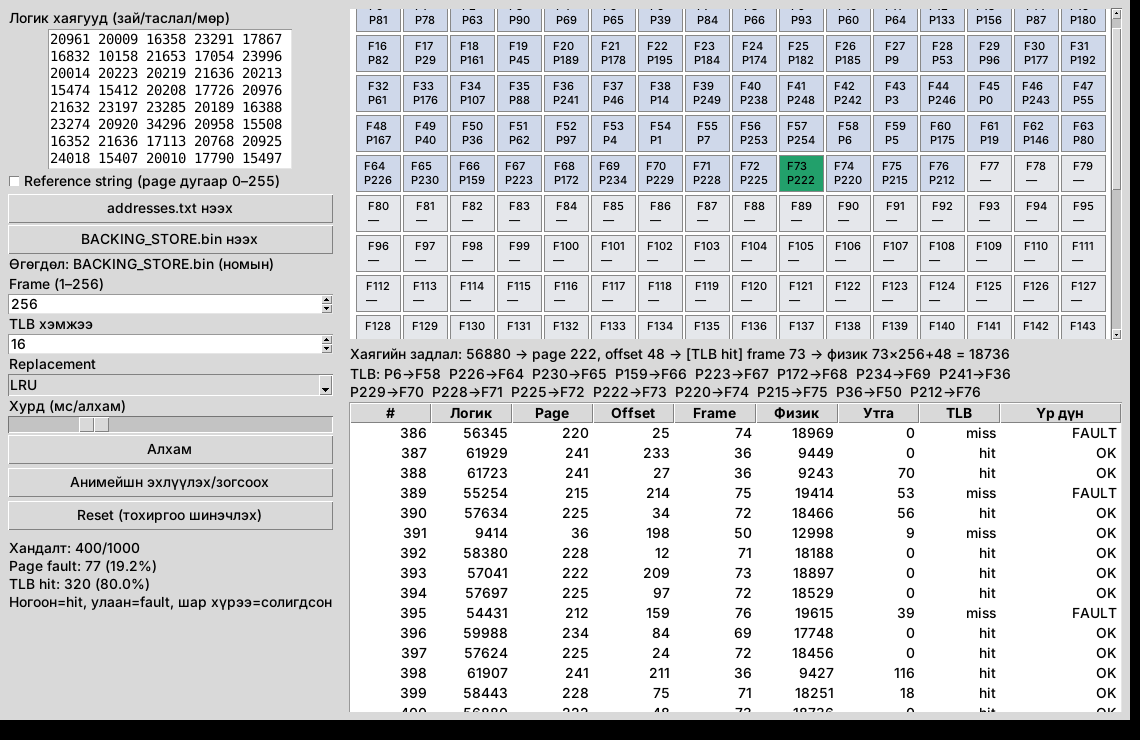
\includegraphics[width=0.93\linewidth]{gui_big.png}};
\begin{scope}[x={(img.south east)}, y={(img.north west)}]
\callout{-0.022}{0.88}{1} \callout{-0.022}{0.62}{2} \callout{-0.022}{0.35}{3} \callout{-0.022}{0.21}{4}
\callout{0.33}{0.96}{5} \callout{0.975}{0.523}{6} \callout{0.975}{0.478}{7} \callout{0.33}{0.40}{8}
\end{scope}
\end{tikzpicture}}
